\documentclass[a5paper,oneside]{amsart}
\usepackage[scale={.9,.9}]{geometry}
\usepackage{mathrsfs}
\usepackage{dsfont}
\theoremstyle{plain}
\usepackage{graphicx}
\newtheorem{theorem}{Theorem}
\newtheorem{lemma}{Lemma}
\newtheorem{corollary}{Corollary}
\newtheorem{proposition}{Proposition}
\newtheorem{conjecture}{Conjecture}
\theoremstyle{definition}
\newtheorem{problema}{Problema}
\newtheorem{ejercicio}{Ejercicio}
\newtheorem*{definition}{Definition}
\newtheorem*{remark}{Remark}
\usepackage{listings}
\lstset{
language=R,
basicstyle=%\scriptsize
\ttfamily,
commentstyle=\ttfamily\color{gray},
numbers=none,
numberstyle=\ttfamily\color{gray}\footnotesize,
stepnumber=1,
numbersep=5pt,
backgroundcolor=\color{white},
showspaces=false,
showstringspaces=false,
showtabs=false,
frame=none,
tabsize=4,
captionpos=b,
breaklines=true,
breakatwhitespace=false,
title=\lstname,
escapeinside={},
keywordstyle={},
morekeywords={}
}
\title[Problemas de Procesos I]{Problemas de Procesos Estoc\'asticos I\\ Semestre 2013-II\\ Posgrado en Ciencias Matem\'aticas\\ Universidad Nacional Aut\'onoma de M\'exico\\TAREA 3}
\author{Antonio Soriano Flores}
%\address{}
\usepackage[colorlinks,citecolor=blue,urlcolor=blue]{hyperref}
\input{definitions.tex}
%\usepackage[colorlinks,citecolor=blue,urlcolor=blue]{hyperref}
\begin{document}
\maketitle




\begin{problema}
Sea $M$ una $\paren{\F_n}$-martingala. Pruebe que si $T$ es un tiempo de paro finito entonces $\esp{M_T}=\esp{M_0}$ bajo cada una de las siguientes condiciones:
\begin{enumerate}
\item $M$ es acotada.
\item $T$ es integrable y la sucesi\'on $\paren{M_n-M_{n-1}}$ es acotada.
\item $\paren{M_{n\wedge T}}$ es uniformemente integrable. 
\end{enumerate}
\begin{proof}
\begin{enumerate}
	\item Supongamos que $M_n$ es acotada, es decir $\abs{M_n}< K$ para toda n.
	Consideremos el tiempo de paro acotado $T \wedge n$, entonces por el Teorema 1.3 de las notas  
	$$
	\esp{M_{T \wedge n}}=\esp{M_0}
	$$
	Como $M_{T \wedge n} \rightarrow M_T$ y como por hip\'otesis M es acotada entonces usando T.C.D. tenemos
	$$
	\esp{M_T}=\esp{\lim_{n \rightarrow \infty}M_{T \wedge n}}=\lim_{n \rightarrow \infty}\esp{M_{T \wedge n}}=\lim_{n \rightarrow \infty}\esp{M_0}=\esp{M_0}
	$$
	\item Supongamos que $T$ es integrable y la sucesi\'on $\paren{M_n-M_{n-1}}$ es acotada. Nuevamente definamos $T \wedge n$ el tiempo de paro acotado, y por Teorema 		1.3 de las notas:
	$$
	\esp{M_{T \wedge n}}=\esp{M_0} \Rightarrow \esp{M_{T \wedge n}-M_0}=0 
	$$
	Como:
	$$
	\abs{M_{T\wedge n}-M_0}=\abs{\sum_{i=1}^{T\wedge n}M_i-M_{i-1}}\leq \sum_{i=1}^{T\wedge n}\abs{M_i-M_{i-1}}\leq \sum_{i=}^{T\wedge n} K \leq \paren{T\wedge n}K\leq TK
	$$
	Por lo tanto la sucesi\'on $\phi_n:=\abs{M_{T\wedge n}-M_0}$ es dominada por la funci\'on medible   $TK$  la cual por hip\'otesis es integrable. Entonces usando el teorema de convergencia dominada y recordando que  $M_{T \wedge n} \rightarrow M_T$, tenemos:
	$$
	\esp{M_T-M_0}=\esp{\lim_{n \rightarrow \infty} \paren{M_{T\wedge n}-M_0} }=\lim_{n \rightarrow \infty}\esp{M_{T\wedge n}-M_0 }=\lim_{n \rightarrow \infty}0=0 
	$$
	Por lo tanto:
	$$
	\esp{M_T-M_0}=0 \Rightarrow \esp{M_T}=\esp{M_0}
	$$
	\item Supongamos que $\paren{M_{n\wedge T}}$ es uniformemente integrable. Entonces por teorema 1.8 de las notas  y dado que $M_{T \wedge n} \rightarrow M_T$ se sigue que:
	$$
	M_T \in L_1 \text{ y } M_{T \wedge n} \rightarrow M_T \text { en $L_1$} \Rightarrow \esp{M_{T \wedge n}} \rightarrow \esp{M_T}	
	$$
	Pero nuevamente por Teorema 1.3 de las notas sabemos que $M_{T \wedge n}=M_0$ por lo tanto se sigue que $\esp{M_T}=\esp{M_0}$
 
	
	
\end{enumerate}
\end{proof}
\defin{Categor\'ias: } Muestreo opcional. 
\end{problema}

\begin{problema}
Sea $M$ una $\paren{\F_n}$-martingala con saltos acotados. Sean\begin{esn}
C=\set{\limsup M_n=\liminf M_n\in\re}\quad\text{y}\quad D=\set{\limsup M_n=-\infty\text{ y }\limsup M_n=\infty}.
\end{esn}Pruebe que $\proba{C\cup D}=1$. Deduzca que las caminatas aleatorias centradas con saltos acotados oscilan. Sugerencia: Para cada $K>0$ defina\begin{esn}
T=\min\set{n\geq 0: \abs{M_n}\geq K}
\end{esn}y aplique el teorema de convergencia de martingalas a $M^T$. 

Sea $M$ una caminata aleatoria no trivial con saltos integrables en $-1,0,1,\ldots$ y  media cero. Pruebe que $\proba{M\text{ converge en }\na}=0$ y  concluya que $\liminf M_n=-\infty$ casi seguramente. (Este resultado permitir\'a dar una prueba adicional de que un Galton-Watson cr\'itico se extingue).  Sugerencia: proceda como en el p\'arrafo anterior y pruebe la integrabilidad uniforme de $M_{T\wedge n},n\in\na$.

\defin{Categor\'ias: } Teoremas de convergencia de martingalas
\end{problema}
\begin{proof}
Definamos el siguiente tiempo de paro:
$$
T_k=\min{\set{n>0: M_n\leq -K}}
$$
Notemos que $T_k$ as\'i definido es tiempo  de paro pues el evento $T_k=n$ depende por definici\'on de los primeros $n$ valores de la martingala  $M$ y por tanto es $\F_n$-medible. Luego abreviemos al conjunto $\set{\omega: T_k(\omega)=\infty}$ como $\set{T_k=\infty}$.\\
Como por hip\'otesis tenemos saltos acotados es decir  $\abs{M_i-M_{i-1}} < C$ para alg\'un $C>0$, entonces tenemos:
$$
M_{T_k\wedge n}\geq -K-C  \Rightarrow M_{T\wedge n} + K + C \geq  0 \text{ para toda n}
$$
Pero como $M_{T\wedge n} $ es martingala  (ver ejercicio 4 de la primera tarea), entonces $M_{T\wedge n} + K + C$  es una martingala positiva y por tanto por el teorema 1.4 de las notas se concluye que  $M_{T\wedge n}$   converge. Pero notemos que en el  conjunto  $\set{T_k=\infty}$ se tiene que $M_{T\wedge n}=M_{n}$, de donde concluimos que $M_n$ converge si  $\set{T_k=\infty}$  para alguna $k \in \mathds{Q^+}$. Es decir, hemos concluido que $M_n$ converge si existe $k$ tal que $T_k=\infty$ es decir.
$$
\bigcup_{k \in \mathds{Q^+}}\set{T_k=\infty}=\liminf_n{M_n}>-\infty
$$ 
Por otro lado si estudiamos el complemento de $\bigcup_{k \in \mathds{Q}}\set{T_k=\infty}$ tenemos que:
$$
\set{\bigcup_{k \in \mathds{Q^+}}\set{T_k=\infty}}^c=\bigcap_{k\in \mathds{Q^+}}\set{T_k < \infty}
$$
Es decir que para toda $K \in \mathds{Q^+}$ se tiene que $\set{T_k < \infty}$ por lo que tendiendo $K$ a infinito tendr\'iamos que $\liminf_n{M_n}=\infty$ pues $M_n \leq -K$ para toda $K$. Finalmente repitiendo el argumento pero ahora para el tiempo de paro $S_k=\min{\set{n>0: M_n \geq K}}$ concluimos que $\limsup_n{M_n}=\infty$. Por lo que se concluye que la martingala o converge o oscila. $\p(C\cup D)=1$

Tomando ahora una caminata aleatoria $S_n=\sum_{i=1}^{n}\xi_i$ (no trivial) con saltos acotados concluimos que dicha caminata  oscila pues:
$$
\p(S_n\rightarrow_{n\rightarrow \infty} k)=0  \text{ para toda $k$ }
$$
Es decir la caminata no puede converge a un n\'umero en $\re$ y por tanto aplicando  lo anterior  la caminata oscilar\'a. Solo falta demostrar que en efecto la caminata no puede converger lo cual se sigue de lo siguiente, si $S_n$ converge a un n\'umero entonces debe de existir un $N \in \na$ tal que  la caminata se estabiliza en $k$:
$$
\p(S_N=k,S_{N+1}=k,S_{N+2}=k,\ldots,S_{N+n}=k)$$$$=\p(S_N=k)\p(\xi_{N+1}=0,\xi_{N+2}=0,\ldots,\xi_{N+n}=0)=\p(S_N=k)\p(\xi_{1}=0)^n
$$
Pero como es una caminata no trivial entonces $\p(\xi_{1}=0)<1$, por lo tanto: $$\p(S_N=k)\p(\xi_{1}=0)^n \rightarrow 0$$ de donde se concluye que  la caminata no converge a un numero real, luego entonces la caminata debe de oscilar.\\
Ahora supongamos que $M_n$ es una caminata con saltos integrables es decir: $\abs{M_i-M_{i-1}} < Y$ con $Y \in L_1$. Procediendo de forma similar al parrafo anterior definimos $T_k=\min\set{n>0:\abs{M_n}>k}$, entonces la martingala $M_{T_{k} \wedge n}$  cumple con :
$$
\abs{M_{T_{k}\wedge n}} < k + Y \in L_1
$$
Aqu\'i usaremos un resultado que dice que si $(f_i)$ es una familia de funciones medibles tal que existe $f \in L_1$ que verifica $\abs{f_i} \leq f$ para todo $i \in I$ entonces $\paren{f_i}_{i\in I}$ es uniformemente integrable.\\
En nuestro caso $M_{T_{k}\wedge n}$ cumple con las condiciones del resultado y por tanto  $M_{T_{k}\wedge n}$ es uniformemente integrable.  De aqu\'i se concluye  que la martingala  $M_{T_{k}\wedge n}$ converge (Teorema 1.8 de las notas).  Siguiendo un argumento similar a la prueba del caso de salto acotados tendr\'iamos que en el conjunto $\set{T_k=\infty}$ se tiene que $M_{T_{k}\wedge n}=M_n$ y por tanto la martingala converge si existe $k$ tal que $\set{T_k=\infty}$ y nuevamente en caso contrario  , la martingala oscilara si para toda $k$ se tiene que $\set{T_k < \infty}$.\\
En el caso de una caminata aleatoria con salto integrales en $\set{-1,0,1,2,3...}$ se tiene que dicha  caminata no puede converger a un numero real  ya que  nuevamente se tendr\'ia que tener que los saltos $\xi_i$ tomaran el valor de $0$ infinitamente para tener convergencia, lo cual no sucede en una caminata no trivial, luego entonces la caminata oscilar\'a y por tanto se concluye que $\liminf M_n=-\infty$ casi seguramente.\qedhere
\end{proof}


\begin{problema}
Sean $X_1,X_2,\ldots$ variables aleatorias intercambiables:\begin{esn}
\paren{X_1,\ldots, X_n}\stackrel{d}{=}\paren{X_{\pi_1},\ldots, X_{\pi_n}}
\end{esn}para cada permutaci\'on $\sigma$ de $\set{1,\ldots,n}$. 
\begin{enumerate}
\item Para $\G,\h$ sub$\sigma$-\'algebras de $\F$ definimos a $\G\vee\h=\sag{\G\cup\h}$. Sea \begin{esn}
\G^n=\sag{\imf{f}{X_1,\ldots, X_n}: \fun{f}{\re^n}{\re}\text{ es sim\'etrica}}\vee\sag{X_{n+1},X_{n+2},\ldots}. 
\end{esn}Pruebe que $\G^n,n\geq 1$ es una filtraci\'on al rev\'es. Sea $\G$ su intersecci\'on.
\begin{proof}
Definamos las siguientes $\sigma$-\'algebras:
$$
\F_n:=\sag{\imf{f}{X_1,\ldots, X_n}: \fun{f}{\re^n}{\re}\text{ es sim\'etrica}}
$$
$$
\h_{n+1}:=\sag{X_{n+1},X_{n+2},\ldots}.
$$
Entonces por definici\'on tendr\'iamos que $\G^n=\sigma(\F_n\cup \h_{n+1})$. Pero notemos que $\F_{n+1} \subset \F_n$ pues si una funci\'on es sim\'etrica en $\re^{n+1}$ tambi\'en lo es en $\re^n$. Sea $\fun{f_{n+1}}{\re^{n+1}}{\re}$ sim\'etrica entonces definimos $\fun{f_n}{\re^n}{\re}$ como $f_n(x_1\ldots x_n)=f_{n+1}(x_1,\ldots x_n,0)$  y al ser $f_{n+1}$ una funci\'on sim\'etrica se sigue que $f_n$ tambi\'en lo es. \\
Por otro lado tambi\'en es claro que por definici\'on:
$$
\h_{n+2} =\sag{X_{n+2},X_{n+3},\ldots} \subset  \sag{X_{n+1},X_{n+2},\ldots} = \h_{n+1}
$$
Entonces como $\F_{n+1} \subset \F_n$ y $\h_{n+2} \subset \h_{n+1}$ para toda $n$.
$$
\F_{n+1} \subset \F_n \Rightarrow \F_{n+1}\cup \h_{n+2}   \subset \F_n  \cup \h_{n+2} \subset \F_n\cup  \h_{n+1}
$$
Entonces  aplicando el operador $\sigma(.)$
$$
\G^{n+1}:=\sigma( \F_{n+1}\cup \h_{n+2}) \subset \sigma(\F_n\cup  \h_{n+1}):=\G^n
$$
Por lo tanto tenemos que $\G^n$ es una filtraci\'on al rev\'es
\end{proof}
\item Para cada $A\in\mc{B}_{\re}$, defina a\begin{esn}
\imf{\Xi_n}{A}=\frac{1}{n}\sum_{i=1}^n \indi{X_i\in A}.
\end{esn}Pruebe que\begin{esn}
\probac{X_1\in A}{\G^n}=\imf{\Xi_n}{A}. 
\end{esn}?`Por qu\'e puede definir a  $\imf{\Xi}{A}=\lim_{n\to\infty}\imf{\Xi_n}{A}$?
\begin{proof}
Sabemos que $X_1,X_2,\ldots, $ son intercambiables. Definamos las siguientes variables:
$$
Y_1=\mathds{1}_{\set{X_1 \in A}},Y_2=\mathds{1}_{\set{X_2 \in A}},\ldots Y_n=\mathds{1}_{\set{X_n \in A}},\ldots
$$
Entonces por definici\'on cada $Y_i \in \set{0,1}$ y son intercambiables pues:
$$
\p(Y_1=i_1,\ldots ,Y_n=i_n)=\p(\mathds{1}_{\set{X_1 \in A}}=i_1,\ldots , \mathds{1}_{\set{X_n \in A}}=i_n)
$$
$$
=\p(\mathds{1}_{\set{X_{\pi(1)} \in A}}=i_1,\ldots , \mathds{1}_{\set{X_{\pi(n)} \in A}}=i_n)= \p(Y_{\pi(1)}=i_1,\ldots ,Y_{\pi(n)}=i_n)
$$
Ahora recordemos la proposici\'on (1.9) de las notas que nos dice que para cualquier funci\'on h medible:
$$
\espc{h(Y_1,\ldots,Y_n)}{\G_n}=\espc{h(Y_{\pi(1)},\ldots,Y_{\pi(n)})}{\G_n}
$$
Entonces tomando $h:\re^n \rightarrow \re$  como $h(Y_1,\ldots,Y_n)=Y_1$ tenemos que:
$$
\espc{Y_j}{\G_n}=\espc{Y_1}{\G_n} \text{ para toda $j \leq n$ }
$$
Por otro lado dado que la funci\'on $f(Y_1,\ldots,Y_n)=\frac{1}{n}\sum_{i=1}^{n}Y_i$ es sim\'etrica se sigue que $\frac{1}{n}\sum_{i=1}^{n}Y_i$ es $\G^n$-medible y por lo tanto:
$$
 \frac{1}{n}\sum_{i=1}^{n}Y_i=\espc{\frac{1}{n}\sum_{i=1}^{n}Y_i}{\G^n}=\frac{1}{n}\sum_{i=1}^{n}\espc{Y_i}{\G^n}=\espc{Y_1}{\G^n}
$$
De donde se concluye que:
$$
\imf{\Xi_n}{A}:= \frac{1}{n}\sum_{i=1}^{n}\mathds{1}_{X_i\in A}=\espc{\mathds{1}_{X_1 \in A}}{\G^n}=\p(X_1 \in A| \G^n)
$$
Qu\'e pasa cuando n tiende a infinito?, para responder esto definamos la siguiente martingala reversa:
$$
M_n=\espc{Y_1}{\G^n}=\frac{1}{n}\sum_{i=1}^{n}\mathds{1}_{X_i\in A}
$$
Por construcci\'on se tiene que $M_n$ cumple con estar en $L_1$ y ser $\G^n$ medible pues:
$$
\esp{\abs{M_n}}=\esp{\abs{\espc{Y_1}{\G^n}}}\leq \esp{\espc{\abs{Y_1}}{\G^n}} =\esp{\abs{Y_1}} < \infty
$$
Por otro lado como:
$$
\espc{M_n}{\G^{n+1}}=\espc{\frac{1}{n}\sum_{i=1}^{n}\mathds{1}_{X_i\in A}}{\G^{n+1}}=\frac{1}{n}\sum_{i=1}^{n}\espc{Y_i}{\G^{n+1}}
$$
$$
=\espc{Y_1}{\G^{n+1}}:=M_{n+1}
$$
Por  lo tanto se puede afirmar que $M_n$ es martingala reversa. Luego por teorema (1.13) de las notas $M_n$ es uniformemente integrable y por tanto  converge casi seguramente y en $L_1$ a $M_{\infty}=\espc{Y_1}{\G^\infty}=\espc{Y_1}{\G}=\lim_{n \rightarrow \infty} \frac{1}{n}\sum_{i=1}^{n}\mathds{1}_{X_i\in A}$.\\
Por lo tanto se puede definir $\imf{\Xi}{A}=\lim_{n\to\infty}\imf{\Xi_n}{A}$, de hecho como tenemos convergencia en $L_1$ y como $\imf{\Xi}{A}$ debe de ser $\G^\infty$-medible ($\sigma$-algebra cola) entonces dicho limite debe de ser una constante, luego como la esperanza de una constante es la constante misma tenemos que:
$$
\imf{\Xi}{A}=\esp{\lim_{n \rightarrow \infty} \frac{1}{n}\sum_{i=1}^{n}\mathds{1}_{X_i\in A}}=\esp{\espc{Y_1}{\G}}=\esp{Y_1}=\esp{\mathds{1}_{\set{X_1 \in A}}}=\p(X_1 \in A)
$$
\end{proof}


\item Al considerar a la martingala\begin{esn}
\frac{1}{n\paren{n-1}}\sum_{1\leq i<j\leq n}\indi{X_i\in A}\indi{X_j\in A},
\end{esn}pruebe que $\probac{X_1\in A,X_2\in A}{\G}=\probac{X_1\in A}{\G}\probac{X_2\in A}{\G}$. Extienda la afirmaci\'on de independencia condicional anterior a $X_1,\ldots, X_n$. 
\begin{proof}
En el inciso anterior probamos que:
$$
\p(X_1 \in A|\G)=\espc{\mathds{1}_{X_1 \in A}}{\G}=\espc{Y_1}{\G}=\lim_{n \rightarrow \infty}\frac{1}{n}\sum_{i=1}^{n}{\mathds{1}_{X_i \in A}}
$$
Repitiendo la demostraci\'on pero ahora tomando $h(Y_1,\ldots,Y_n)=Y_2$ obtenemos que:
$$
\p(X_2 \in A|\G)=\espc{\mathds{1}_{X_2 \in A}}{\G}=\espc{Y_2}{\G}=\lim_{n \rightarrow \infty}\frac{1}{n}\sum_{i=1}^{n}{\mathds{1}_{X_i \in A}}
$$ 
Por otro lado notemos que $f(Y_1,\ldots,Y_n)=\frac{1}{n\paren{n-1}}\sum_{1\leq i \neq j\leq n}Y_iY_j$ es sim\'etrica se sigue que $\frac{1}{n\paren{n-1}}\sum_{1\leq i \neq j\leq n}Y_iY_j$ es $\G^n$-medible y por lo tanto:
$$
\frac{1}{n\paren{n-1}}\sum_{1\leq i \neq j\leq n}Y_iY_j=\espc{\frac{1}{n\paren{n-1}}\sum_{1\leq i \neq j\leq n}Y_iY_j}{\G^n}=\espc{Y_1Y_2}{\G^n}
$$
de donde se observa que en efecto:
$$
M_n=\frac{1}{n\paren{n-1}}\sum_{1\leq i \neq j\leq n}Y_iY_j \text{    con  $n > 1$ }
$$
Es una martingala reversa y por tanto converge casi seguramente y en $L_1$. En este caso la martingala converge a $M_\infty=\espc{Y_1Y_2}{\G^\infty}=\espc{Y_1Y_2}{\G}$. Por lo tanto tenemos lo siguiente:
$$
\p(X_1 \in A, X_2 \in A|\G)=\espc{Y_1Y_2}{\G}=M_\infty=\lim_{n \rightarrow \infty}\frac{1}{n\paren{n-1}}\sum_{1\leq i \neq j\leq n}Y_iY_j 
$$
Ahora observemos lo siguiente:
$$
\paren{\sum_{i=1}^{n}{Y_i}}\paren{\sum_{j=1}^{n}{Y_j}}=\sum_{i=1}^{n}Y_i^2+\sum_{1\leq i \neq j\leq n}Y_iY_j 
$$
De donde despejando:
$$
\sum_{1\leq i \neq j\leq n}Y_iY_j =\paren{\sum_{i=1}^{n}{Y_i}}\paren{\sum_{j=1}^{n}{Y_j}}-\sum_{i=1}^{n}Y_i^2
$$
Pero $Y_i^2=\paren{\mathds{1}_{X_i \in A}}^2=\mathds{1}_{X_i \in A}=Y_i$. Entonces:
$$
\sum_{1\leq i \neq j\leq n}Y_iY_j =\paren{\sum_{i=1}^{n}{Y_i}}\paren{\sum_{j=1}^{n}{Y_j}-1}
$$
Por lo tanto tomando limite
$$
\lim_{n \rightarrow \infty}\frac{1}{n\paren{n-1}}\sum_{1\leq i \neq j\leq n}Y_iY_j =\lim_{n \rightarrow \infty}\frac{1}{n\paren{n-1}}\paren{\sum_{i=1}^{n}{Y_i}}\paren{\sum_{j=1}^{n}{Y_j}-1}
$$
$$
\lim_{n \rightarrow \infty}\frac{\sum_{i=1}^{n}{Y_i}}{n}\paren{\frac{\sum_{i=1}^{n}{Y_i}}{n-1}-\frac{1}{n-1}}=\lim_{n \rightarrow \infty}\paren{\frac{\sum_{i=1}^{n}{Y_i}}{n}}\paren{\paren{\frac{\sum_{i=1}^{n}{Y_i}}{n}}\paren{\frac{n}{n-1}}-\frac{1}{n-1}}
$$
Como los limites de los factores existe, entonces:
$$
\paren{\lim_{n \rightarrow \infty}\frac{\sum_{i=1}^{n}{Y_i}}{n}}\paren{\paren{\lim_{n \rightarrow \infty}\frac{\sum_{i=1}^{n}{Y_i}}{n}}\paren{\lim_{n \rightarrow \infty}\frac{n}{n-1}}-\paren{\lim_{n \rightarrow \infty}\frac{1}{n-1}}}
$$
$$
\paren{\lim_{n \rightarrow \infty}\frac{\sum_{i=1}^{n}{Y_i}}{n}}\paren{\lim_{n \rightarrow \infty}\frac{\sum_{i=1}^{n}{Y_i}}{n}}=\p(X_1 \in A|\G)\p(X_2 \in A|\G)
$$
Por lo tanto obtenemos:
$$
\probac{X_1\in A,X_2\in A}{\G}=\probac{X_1\in A}{\G}\probac{X_2\in A}{\G}
$$
Ahora generalizaremos el resultado para para $X_1, \ldots X_k$. Para ello tomaremos la martingala
$$
M_n=\frac{1}{n(n-1)\ldots (n-(k-1)}\sum_{1\leq i_1 \neq i_2 \ldots \neq i_k \leq n}Y_{i_1}Y_{i_2}\ldots Y_{i_k}
$$
El cual al ser $f(Y_1 \ldots Y_k)=\frac{1}{n(n-1)\ldots (n-(k-1)}\sum_{1\leq i_1 \neq i_2 \ldots \neq i_k \leq n}Y_{i_1}Y_{i_2}\ldots Y_{i_k}$ una funci\'on sim\'etrica $(n>k)$ entonces se sigue que:
$$
M_n=\espc{Y_1Y_2\ldots Y_k}{\G^n}
$$
Es una martingala reversa y por tanto convergente casi seguramente y en $L_1$, es decir :
$$
M_\infty=\espc{Y_1Y_2\ldots Y_k}{\G}=\probac{X_1 \in A, X_2 \in A, \ldots,X_k \in A}{\G}
$$
Por lo que ahora habria que  probar que:
$$
\lim_{n \rightarrow \infty}\frac{1}{n(n-1)\ldots (n-(k-1)}\sum_{1\leq i_1 \neq i_2 \ldots \neq i_k \leq n}Y_{i_1}Y_{i_2}\ldots Y_{i_k}
$$
$$
=\paren{\lim_{n \rightarrow \infty}\frac{1}{n}\sum_{i=1}^{n}Y_i}^k=\p(X_1 \in A|\G)\p(X_2 \in A|\G) \ldots \p(X_k \in A|\G)
$$
Faltar\'ia probar esto \'ultimo :(
\end{proof}
\end{enumerate}

\defin{Cagegor\'ias: }Teorema de convergencia de martingalas, teorema de de Finetti.
\end{problema}

\begin{ejercicio}
\mbox{}
\begin{enumerate}
\item Ejecute y explique la funci\'on del siguiente c\'odigo en Octave. Comente qu\'e teoremas del curso (y del curso de probabilidad) son importantes para interpretar la figura.
\begin{lstlisting}
	tic;
	n =1000;
	m =10000;
	u= rand (n,m);
	r=2;
	v=3;
	c=1;
	x= ones (1,m)*(r/(r+v));
	for i=1:n
		x(i+1 ,:) =(r+v+(i -1)*c)/(r+v+i*c).*x(i ,:) +(u(i ,:) <x(i,:))./(r+v+i*c);
	endfor
	y= sort (x(n+1 ,:));
	plot (y ,(1: m)./m,y, betacdf (y,r/c,v/c))

\end{lstlisting}
\begin{figure}
  \centering
    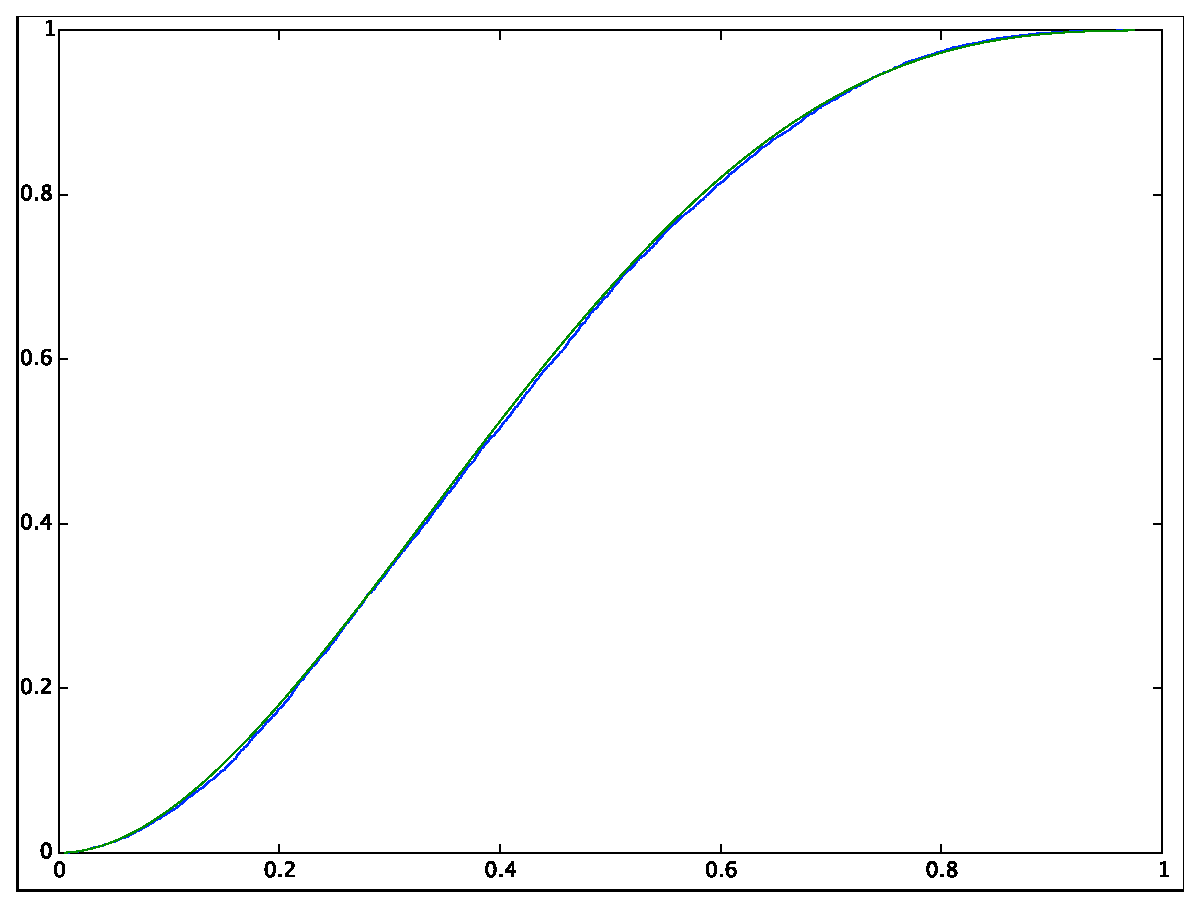
\includegraphics[width=0.7\textwidth]{PoylaBeta.eps}
  \caption{Grafica 1}
  \label{fig:ejemplo}
\end{figure}
El c\'odigo  que nos proporcionan es sobre el problema de las urnas de poyla. En clase vimos que la proporci\'on de bolas rojas  era una martingala adem\'as al ser positiva se concluy\'o que dicha variable converg\'ia casi seguramente  a una variable $X_\infty$. De hecho en la tarea $1$ se simul\'o este proceso y se observaba que en efecto la trayectoria se estabilizaba conforme $n$ se iba a infinito. \\
Dado que $X_\infty$ es una variable aleatoria, surgi\'o entonces la pregunta de saber cu\'al era su distribuci\'on. Fue con ayuda del teorema de  De Finetti y la intercambiabilidad que se logr\'o probar que la variable $X_\infty$ ten\'ia exactamente los mismos momentos que una distribuci\'on Beta  de par\'ametro $\paren{\frac{r}{c},\frac{v}{c}}$.\\
El c\'odigo anterior lo que esta haciendo entonces es simular $10,000$ trayectorias del proceso en donde en cada trayectoria se est\'an generando $1,000$  realizaciones del experimento. Al final lo que vemos es un par de gr\'aficas en donde se muestra que en efecto, la distribuci\'on emp\'irica que genera la simulaci\'on es pr\'acticamente igual a la distribuci\'on de un a Beta, por lo tanto se verifica la convergencia de la martingala a una variable $X_\infty$ con distribuci\'on beta.


\item Ejecute y explique la funci\'on del siguiente c\'odigo en Octave. Incluya una gr\'afica en la que la longitud de la variable k sea mayor a 1000. (Puede modificar el programa...) En la gr\'afica observara un esbozo de la trayectoria de un proceso de ramificaci\'on continuo (en una escala distinta...).
\begin{lstlisting}
k =[10];
aux=k( length (k));
while (aux >0 && length (k) <1000)
k=[k;2* binornd (aux ,.5) ];
aux=k( length (k));
endwhile
plot (k)
\end{lstlisting}
\end{enumerate}
\end{ejercicio}
Lo que el c\'odigo esta simulando es un proceso de Galton-Watson, el proceso inicia con una  poblaci\'on de 10 sujetos luego cada sujeto puede tener $2$ o $0$  hijos con probabilidad $1/2$, esto quiere decir que la distribuci\'on de  progenia est\'a dada por $\p(X=0)=1/2=\p(X=2)$. Luego entonces la media $\esp{X}=1$ por lo que estamos en el "caso critico" y por tanto sabemos que la poblaci\'on se extinguira\'a con probabilidad 1.  Las simulaciones terminan cuando la \'ultima generaci\'on es de $0$ sujetos. El ejercicios nos pide que veamos una gr\'afica en donde la longitud de k sea mayor a 1000, es decir una trayectoria en donde la poblaci\'on se extinga despu\'es de la generaci\'on  1000, para ello utilizamos el siguiente c\'odigo:
\begin{lstlisting}
k =[10];
aux = k(length(k));
while length(k)<1000
    k =[10];
    aux = k(length(k));
    while (aux > 0)
        k =[k;2*binornd(aux,.5)];
        aux =k(length(k));
    endwhile
endwhile
plot(k)
\end{lstlisting}
\begin{figure}
  \centering
    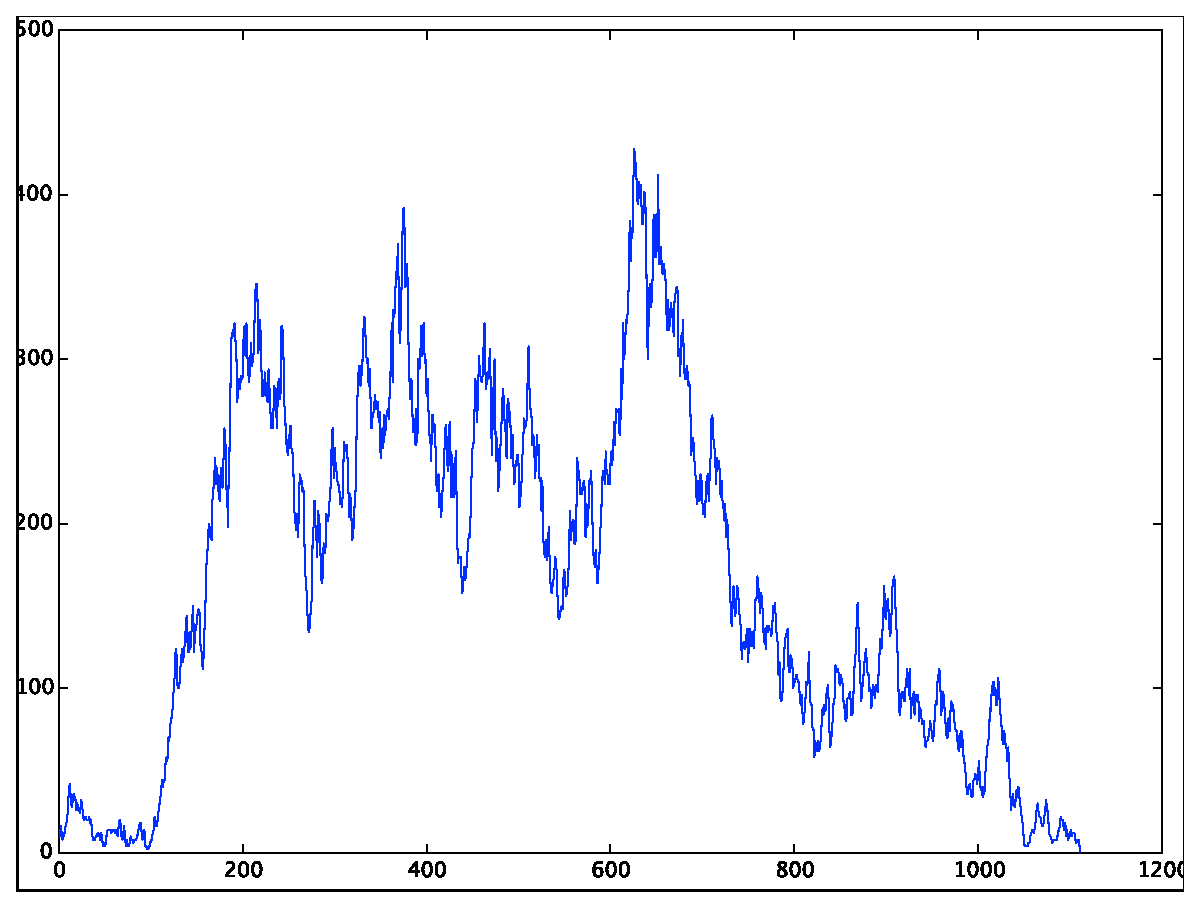
\includegraphics[width=0.7\textwidth]{GaltonWatson.eps}
  \caption{Grafica 2}
  \label{fig:ejemplo}
\end{figure}
%
%\begin{problema}
%Sean $\F_1,\F_2,\ldots $ y $\G$ sub\sa s de $\F$. Decimos que $\F_1,\F_2,\ldots$ son condicionalmente independientes dada $\G$ si para cualquier $H_i$ que sea $\F_i$ medible y acotada se tiene que\begin{esn}
%\espc{H_1\cdots H_n}{\G}=\espc{H_1}{\G}\cdots \espc{H_n}{\G}.
%\end{esn}
%\begin{enumerate}
%\item ?`Qu\'e quiere decir la independencia condicional cuando $\G=\set{\oo,\emptyset}$?
%\item Pruebe que $F_1$ y $\F_2$ son condicionalmente independientes dada $\G$ (denotado $\condind{\F_1}{\F_2}{\G}$) si y s\'olo si para cualquier $H$ que sea $\F_1$-medible y acotada se tiene que\begin{esn}
%\espc{H}{\F_2,\G}=\espc{H}{\G}.
%\end{esn}
%\item Pruebe que $\F_1,\F_2,\ldots, $ son condicionalmente independientes dada $\G$ si y s\'olo si para cada $n\geq 1$, $\F_{n+1}$ es condicionalmente independiente de $\F_1,\ldots, \F_n$ dada $\G$. 
%\end{enumerate}
%
%\defin{Categor\'ias: } Esperanza condicional, Independencia condicional.
%\end{problema}
%
%\begin{problema}
%Sea $\mu$ una distribuci\'on de progenie y defina $\tilde \mu_j=\mu_{j+1}$. Sea $S=\paren{S_n}$ una caminata aleatoria con distribuci\'on de salto $\tilde\mu$. Sea $k$ un entero no-negativo y defina recursivamente\begin{esn}
%Z_0=k=C_0,\quad Z_{n+1}=k+S_{C_n}\quad\text{y} C_{n+1}=C_n+Z_{n+1}.
%\end{esn}
%\begin{enumerate}
%\item Pruebe que $Z_n\geq 0$ para toda $n$ y que si $Z_n=0$ entonces $Z_{n+1}=0$.
%\item Pruebe que $C_n$ es un tiempo de paro para la filtraci\'on can\'onica asociada a $S$.
%\item Pruebe que $Z$ es un proceso de Galton-Watson con ley de progenie $\mu$. 
%\item Pruebe que si $S$ alcanza $-1$ entonces existe $n$ tal que $Z_n=0$. Deduzca que si la media de $\mu$ es $1$ entonces $Z$ se extingue. (Sugerencia: utilice un ejercicio anterior sobre martingalas con saltos acotados hacia abajo.) 
%\end{enumerate}
%
%\defin{Categor\'ias: } Caminatas aleatorias, Procesos de Galton-Watson%, Propiedad de Markov fuerte.
%\end{problema}
%
%\begin{problema}
%Sea $\mu$ una distribuci\'on de progenie y defina $\tilde \mu_j=\mu_{j+1}$. Sea $\nu$ una distribuci\'on en $\na$. Consideremos a dos caminatas aleatorias $S=\paren{S_n}$  y $T$ con  distribuci\'ones de salto $\tilde\mu$ y $\nu$.
%\begin{enumerate}
%\item ?`Qu\'e significa que $S$ y $T$ sean independientes? As\'umalo.
%\item Sea $k$ un entero no-negativo y defina recursivamente\begin{esn}
%Z_0=k=C_0,\quad Z_{n+1}=k+S_{C_n}+T_n\quad\text{y} C_{n+1}=C_n+Z_{n+1}.
%\end{esn}
%\item Pruebe que $Z_n\geq 0$ para toda $n$.
%\item Pruebe que $C_n=k\in\F^S_k\cap\F^T_n$.
%\item Pruebe que $Z$ es un proceso de Galton-Watson con inmigraci\'on.
%\end{enumerate}
%
%\defin{Categor\'ias: } Caminatas aleatorias, Procesos de Galton-Watson, Construcci\'on de procesos estoc\'asticos
%\end{problema}
%
%\begin{problema} %Construcci\'on tipo Poisson 
%Sean $\mu$ y $\nu$ una distribuci\'on de progenie y de inmigraci\'on. Sean $Y_1,Y_2,\ldots$ independientes y de ley $\nu$. Suponga que condicionalmente a $Y$, $X^0,X^1,X^2,\ldots$ son procesos de Galton-Watson independientes tales que $X^0_0=k$ y $X^k_0=Y_k$ para $k\geq 1$. Pruebe que si\begin{esn}
%Z_n=\sum_{k=0}^n X^k_{n-k},
%\end{esn}entonces $Z$ es un proceso de Galton-Watson con distribuciones de progenie e inmigraci\'on $\mu$ y $\nu$ que comienza en $k$. 
%
%\defin{Categor\'ias: } Procesos de ramificaci\'on
%\end{problema}
%
%\begin{problema}
%Para cada par de medidas de probabilidad en $\na^\na$ $\p_1$ y $\p_2$ definimos a la convoluci\'on de $\p_1$ y $\p_2$, denotada $\p_1 *\p_2$, como la distribuci\'on de $\paren{S^1_k+S^2_k,k\geq 0}$ donde $S^1$ y $S^2$ son independientes y de distribuciones $\p_1$ y $\p_2$ respectivamente.
%\begin{enumerate}
%\item ?` Cu\'al es la relaci\'on entre las distribuciones finito-dimensionales de $\p_1$, $\p_2$ y $\p_1*\p_2$?
%\item Sea $\p_k^\mu$ la distribuci\'on de un proceso de Galton-Watson  de ley de reproducci\'on $\mu$ que comienza en $k$. Pruebe que $\p_{k_1}*\p_{k_2}=\p_{k_1+k_2}$.
%%\item Caracterizaci\'on de leyes markovianas con la propiedad de ramificaci\'on.
%\end{enumerate}
%
%\defin{Categor\'ias: } Distribuciones finito-dimensionales, Procesos de ramificaci\'on.
%\end{problema}
\bibliography{GenBib}
\bibliographystyle{amsalpha}
\end{document}